%%%%%%%%%%%%%
\chapter{Ergebnisdiskussion}
\label{ch:Results}
%%%%%%%%%%%%%
Zur Formulierung des \emph{TMA} werden die in Kapitel \ref{ch:evaluation} beschriebenen Daten zunächst interpretiert. Die Ergebnisse der Interpretation werden kritisch betrachtet und, basierend auf der Ergebnisinterpretation, der daraus resultierende \emph{TMA} beschrieben. 


\section{Ergebnisinterpretation}
Die Ergebnisinterpretation erfolgt auf den, in Kapitel \ref{ch:evaluation}, aufgestellten Hypothesen. Die Ergebnisse werden kategorisiert betrachtet. Gegenübergestellt werden jeweils, wie bisher, das Konstruktionsprinzip und Konfigurationsprinzip, sowie der Einsatz von Sprüngen und die Verwendung von Sichtbarkeitsregeln. Die Betrachtung der Ergebnisse wird gemäß der zuvor verwendeten Reihenfolge erfolgen. Abschließend werden die Ergebnisse zusammengefasst dargestellt.


\subsection{Konfigurationsprinzip und Konstruktionsprinzip}



\begin{figure}
   \begin{minipage}[b]{.49\linewidth} % [b] => Ausrichtung an \caption
      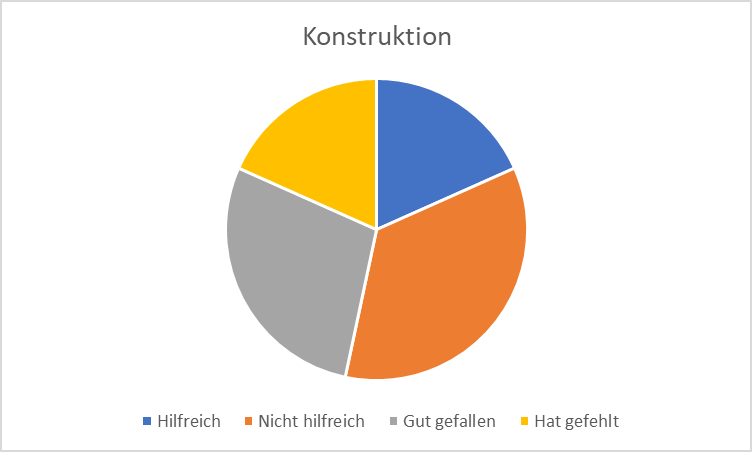
\includegraphics[width=\linewidth]{pictures/diagramme/aussagenkonstr}
      \caption{Wasser}
   \end{minipage}
   \hspace{.01\linewidth}% Abstand zwischen Bilder
   \begin{minipage}[b]{.49\linewidth} % [b] => Ausrichtung an \caption
      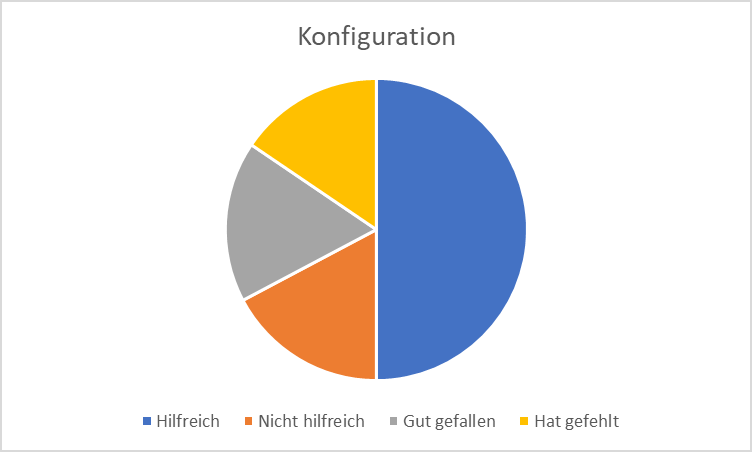
\includegraphics[width=\linewidth]{pictures/diagramme/aussagenkonfig}
      \caption{Land}
   \end{minipage}
\end{figure}

\paragraph{Verständlichkeit der Triggereinstellungen}
Die Bewertung der Fragebogenergebnisse zeigen auf, dass die Triggereinstellungen des \emph{TherapyBuilder}-Prototyps für die Probanden verständlicher ist.

%\paragraph{Verständlichkeit der Triggereinstellungen}
%Die direkte Bindung von Bedingungen (Conditions) und Auslösern (Triggern) sowie deren Einstellungen an eine Konversation wirkt sich positiv auf die Verständlichkeit der Triggereinstellungen aus. 
%
%Dem entgegen steht die Anordnung von Auslösern (Triggern) und Bedingungen (Conditions) in Verschachtelungen, mit beliebig vielen Bezügen zu Konversationen.


\paragraph{Verständlichkeit der Triggerdarstellung}
\paragraph{Übersichtlichkeit der Konversationen}
\paragraph{Übersichtlichkeit der zeitlichen Darstellung der Konversationen}
\paragraph{Verständlichkeit der Triggerkonfiguration}
\paragraph{Übersichtlichkeit der Therapie}
\paragraph{Verständlichkeit von Abhängigkeiten zwischen Konversationen und Konversationsverzweigungen}




\subsection{Sprünge und Sichtbarkeitsregeln}

\begin{figure}
   \begin{minipage}[b]{.49\linewidth} % [b] => Ausrichtung an \caption
      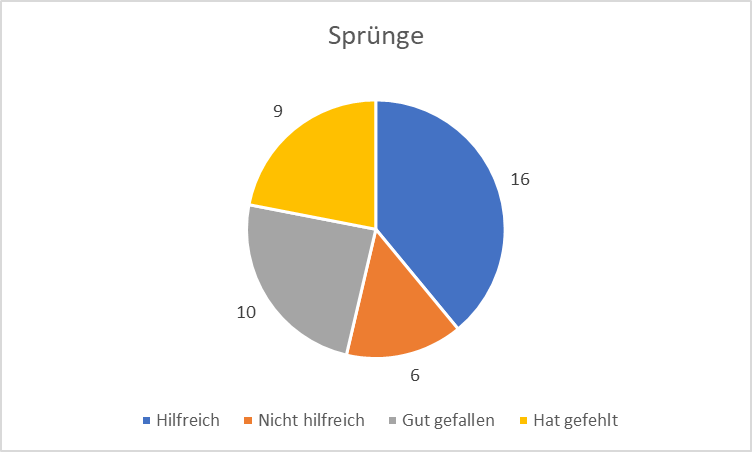
\includegraphics[width=\linewidth]{pictures/diagramme/aussagenspr}
      \caption{Wasser}
   \end{minipage}
   \hspace{.01\linewidth}% Abstand zwischen Bilder
   \begin{minipage}[b]{.49\linewidth} % [b] => Ausrichtung an \caption
      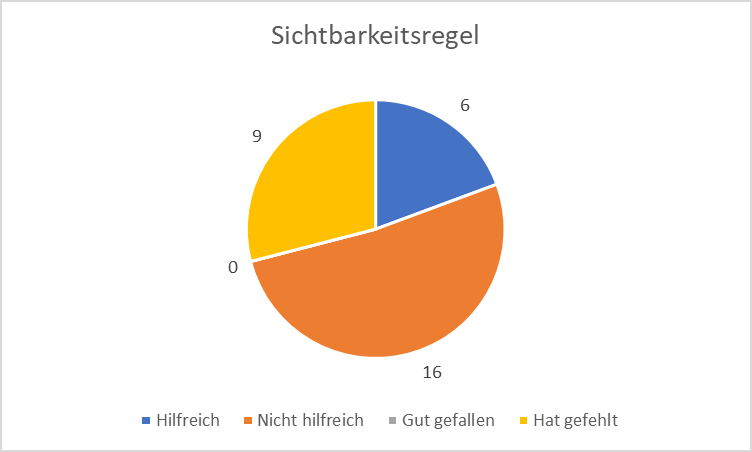
\includegraphics[width=\linewidth]{pictures/diagramme/aussagensichtb}
      \caption{Land}
   \end{minipage}
\end{figure}

\paragraph{Verständlichkeit der Konversationsdarstellung}
\paragraph{Verständlichkeit der Konversationseinstellungen}
\paragraph{Übersichtlichkeit des Konversationsverlaufs}
\paragraph{Übersichtlichkeit der Antwortoptionen innerhalb des Konversationsverlaufs}
\paragraph{Verständlichkeit der Verzweigungen innerhalb des Konversationsverlaufs}
\paragraph{Übersichtlichkeit der Werkzeugpalette zur Konversationserstellung}




\subsection{Zusammenfassung}

\section{Kritische Reflexion}

\begin{figure}[h]
\centering
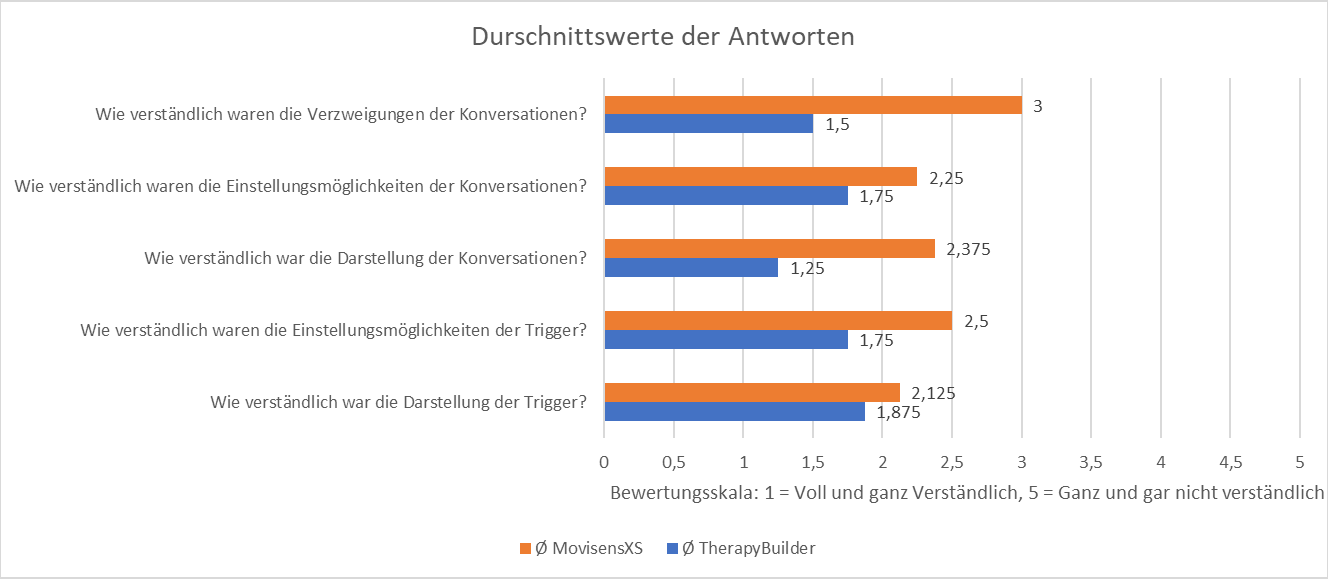
\includegraphics[width=1\textwidth]{pictures/diagramme/antwortendurchsch1}
\caption{Architektur des \emph{konfiguration}}
\label{antwortendurchsch1}
\end{figure}

\begin{figure}[h]
\centering
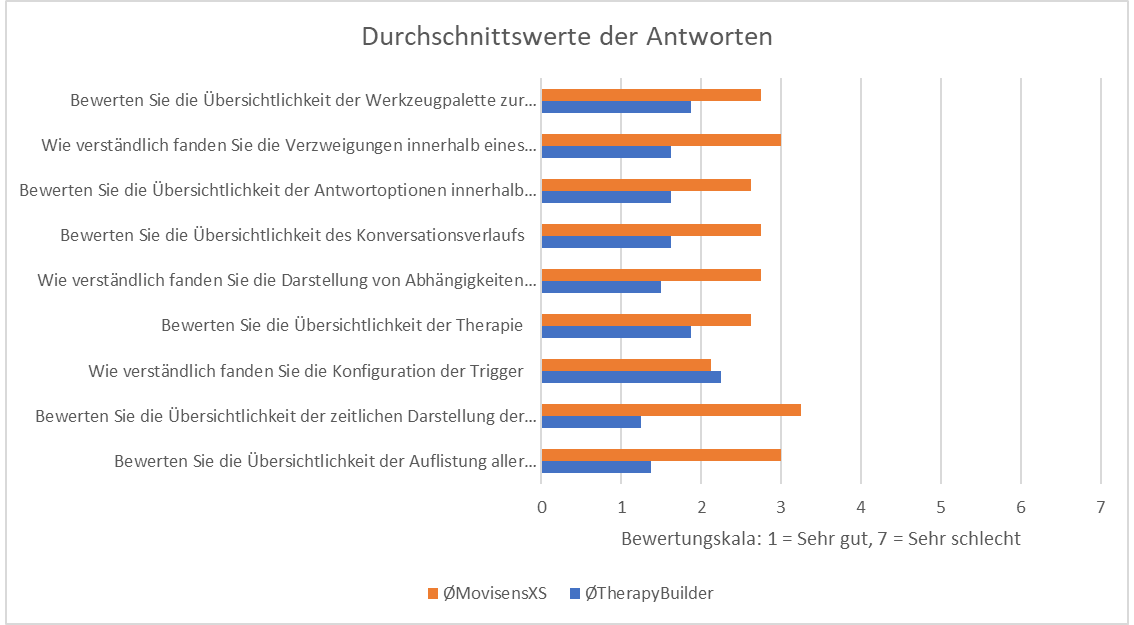
\includegraphics[width=1\textwidth]{pictures/diagramme/antwortendurchsch2}
\caption{Architektur des \emph{konfiguration}}
\label{antwortendurchsch2}
\end{figure}


%Ziel der Arbeit ist die Konzeption eines Therapiemodellierungsansatz (\emph{TMA}). Dieser soll es erlauben, auch technisch wenig versierten Psychologen ihre Therapieideen in einer Art und Weise zu formulieren, die von einer Maschine verarbeitet und ausgeführt werden kann. Dadurch entfällt der hohe und fehleranfällige Abstimmungsaufwand zwischen Forschern und Entwicklern. 


%%%%%%%%%%%%%%%%%%%%%%%%%%%%%%%%%%%%%%%%%%%%%%%%%%%%%%%%%%%%%%%%%%%%%
%%%%%%%%%%%%%%%%%%%%%%%%%%%%%%%%%%%%%%%%%%%%%%%%%%%%%%%%%%%%%%%%%%%%%

%\paragraph{Verständlichkeit der Triggerdarstellung}
%Die im Konfigurationsprinzip verwendete grafische Abbildung der zeitlichen Abläufe, durch Zeitstrahl, farbliche Kodierung, Symbole und Anordnung der Konversationen als Liste verdeutlicht, wirken sich positiv auf die Verständlichkeit der Triggerdarstellung aus. 
%
%Im Vergleich steht das Konstruktionsprinzip, welches die Triggerdarstellung als zeitliche Abläufe grafisch, als Baum und durch die Anordnung von Blöcken, wie Konversationen (Conversations), Auslösern (Triggern) und Bedingungen (Conditions) sowie einer farblicher Kodierung, nach dem Ampelprinzip, und Formen umsetzt.
%
%
%\paragraph{Verständlichkeit der Triggereinstellungen}
%Die direkte Bindung von Bedingungen (Conditions) und Auslösern (Triggern) sowie deren Einstellungen an eine Konversation wirkt sich positiv auf die Verständlichkeit der Triggereinstellungen aus. 
%
%Dem entgegen steht die Anordnung von Auslösern (Triggern) und Bedingungen (Conditions) in Verschachtelungen, mit beliebig vielen Bezügen zu Konversationen.
%
%\paragraph{Übersichtlichkeit der Konversationen}
%Die Darstellung aller vorhandenen Konversationen in Form einer Liste, innerhalb der zeitlichen Darstellung, trägt zur Verbesserung der Übersichtlichkeit der Verwendeten Konversationen bei.
%
%Innerhalb des Konstruktionsprinzips wird die Darstellung aller verwendeten Konversationen, im Samplingbaum in Form von \emph{Conversation}-Blöcke umgesetzt. Diese können beliebig im Baum platziert und angeordnet werden.
%
%\paragraph{Übersichtlichkeit der zeitlichen Darstellung der Konversationen}
%Die im Konfigurationsprinzip verwendete grafische Abbildung der zeitlichen Abläufe, in Form eines Zeitstrahls und durch Anordnung der Konversationen als Liste, trägt zu einer besseren Übersicht der zeitlichen Abfolge von Konversationen bei. 
%
%Im Vergleich steht das Konstruktionsprinzip, welches die zeitliche Abläufe grafisch, als Baum und durch die Anordnung von Blöcken, wie Konversationen (Conversations) und Auslösern (Triggern), umsetzt.
%
%\paragraph{Verständlichkeit der Triggerkonfiguration}
%Die Art der Unterscheidung zwischen Trigger und Condition tragen zur Verständlichkeit der Konfiguration der Triggereinstellungen einer Konversation bei. Hierbei gibt es zwischen Trigger und Condition keine Abhängigkeit. 
%
%Im Gegensatz zum Konfigurationsprinzip setzt das Konstruktionsprinzop eine Unterscheidung zwischen Trigger und Condition innerhalb des Samplingbaums ein. Diese werden durch Blöcke dargestellt, die sich in Farbe, Form und Anordnungsmöglichkeit unterscheiden. Trigger und Conditions sind außerdem voneinander abhängig.
%
%\paragraph{Übersichtlichkeit der Therapie}
%Insgesamt tragen die Verwendeten Stilmittel des Konfigurationsprinzip, zur Übersichtlichkeit einer Therapie, bei. Die Verwendeten Stilmittel sind hierbei die Auflistung der Verwendeten Konversationen, die zeitliche Darstellung dieser in einem Zeitstrahl, Unterscheidung dieser anhand von Farben und Formen sowie Verdeutlichung von Abhängigkeiten zwischen Konversationen durch Linien. 
%
%Dieser Form der Übersicht steht die Darstellung der Therapie in Form eines Baums entgegen. Die Übersicht der Therapie wird hierbei durch Anordnung der Blöcke, deren Farben sowie Inhalte, Verbindungen und Anordnung gegeben. 
%
%
%\paragraph{Verständlichkeit von Abhängigkeiten zwischen Konversationen und Konversationsverzweigungen}
%Die Abbildung der Abhängigkeiten zu anderen Konversationen im Zeitstrahl und der Verzweigung von Konversationen, visualisiert durch Linien, wirkt sich positiv auf die Verständlichkeit von Verzweigungen von Konversationen und Abhängigkeiten zwischen Konversationen aus. 
%
%Diesem Designprinzip steht die Darstellung von  Abhängigkeiten zu anderen Konversationen durch Verzweigungen im Baum und \emph{Check Variable} Blöcke entgegen. 


%%%%%%%%%%%%%%%%%%%%%%%%%%%%%%%%%%%%%%%%%%%%%%%%%%%%%%%%%%%%%%%%%%%%%
%%%%%%%%%%%%%%%%%%%%%%%%%%%%%%%%%%%%%%%%%%%%%%%%%%%%%%%%%%%%%%%%%%%%%


%\subsubsection{Sprünge und Sichtbarkeitsregeln}
%Die verwendeten Sprünge und damit einhergehende Darstellung, wird hinsichtlich dessen Verständlichkeit und Übersichtlichkeit überprüft. Aufgestellt werden Hypothesen, die auf die Darstellung und Einstellung einer Konversation eingehen. Insgesamt werden zum Konzept der Sprünge und dessen Umsetzung sechs Hypothesen aufgestellt, die eine Verbesserung gegenüber der Verwendung von Sichtbarkeitsregeln und der zugehörigen Darstellung messen sollen.
%
%\paragraph{Verständlichkeit der Konversationsdarstellung}
%Die Darstellung einer Konversation, welche mit dem Einsatz von Sprüngen einhergeht, trägt zur besseren Verständlichkeit der Konversationsdarstellung bei. In der Umsetzung werden Chatverläufe in einer Weise dargestellt, die in bekannten Chat-Technologien zum Einsatz kommt. Dies beinhaltet räumliche wie farbliche Trennung der Chatbot-Ausgaben und Nutzer-Eingaben.
%
%Dieser Form der Umsetzung wird die Unterscheidung durch Icons und Textbeschreibung entgegen gestellt.
%
%
%\paragraph{Verständlichkeit der Konversationseinstellungen}
%Das Einbauen eines Elements, welches Variablen überprüft und sich auf mehrere Elemente auswirken kann, trägt zur besseren Verständlichkeit der Einstellung des Konversationsverlaufs bei.
%
%Das Konzept der \emph{Sichtbarkeitsregeln}, welches entgegen gestellt wird, nutzt die Metapher eines Auges. Dieses kann an einer Form aktiviert werden um eine Sichtbarkeitsregel zu hinterlegen. Die Sichtbarkeitsregel bezieht sich nur auf die entsprechende Form. 
%
%\paragraph{Übersichtlichkeit des Konversationsverlaufs}
%Die Verwendung von Spalten, sogenannten \emph{Lanes}, tragen zur Übersicht von Konversationsverzweigungen bei.
%
%
%\paragraph{Übersichtlichkeit der Antwortoptionen innerhalb des Konversationsverlaufs}
%Die Visualisierung von Nutzereingabe innerhalb der Dialogansicht durch den Einsatz der Button-Metapher trägt zur besseren Übersicht der Antwortmöglichkeiten des Nutzers bei.
%
%Diesem Konzept steht die Darstellung der Antwortmöglichkeiten nach öffnen der Einstellungen einer Form entgegen.
%
%
%\paragraph{Verständlichkeit der Verzweigungen innerhalb des Konversationsverlaufs}
%Die Visualisierung von Verzweigungen innerhalb eines Dialogverlaufs mittels Bedingungsblock und Verweis auf Lanes, tragen maßgeblich zur Verständlichkeit bei. Der Nutzer versteht, dass es sich um eine Verzweigung handelt und welche Auswirkungen diese hat. 
%
%Diesem Design steht die Visualisierung von Verzweigungen innerhalb eines Dialogverlaufs mit Sichtbarkeitsregeln entgegen.



%\paragraph{Übersichtlichkeit der Werkzeugpalette zur Konversationserstellung}
%Eine strikte Trennung von Chatbot-Ausgabe und Nutzereingabe trägt maßgeblich zur Übersichtlichkeit der Werkzeugpalette bei. 
%
%Dem steht die Trennung von Chatbot-Ausgabe ohne Erwartung eines Nutzerinputs und Chatbot-Ausgaben mit Erwartung eines Nutzerinputs entgegen, die im \emph{movisensXS}-Prototyp verwendet wird. 